De acuerdo al último reporte en la actualidad publicado por la Comisión de Promoción del Perú para la Exportación y el Turismo (PROMPERÚ). en \citeA{2017PerfilExtranjero} menciona que en el 2017 los turistas extranjeros que visitaron Puno 67\% de los turistas viajan por cuenta propia (sin utilizar los servicios de una agencia de viajes/turismo) como se puede observar en la Figura~\ref{fig:modalidad_viaje_extrajero}. También se observa en la Figura \ref{fig:tiempo_planificacion_extranjero} que su planificación lo hacen con bastante anticipación.
\begin{figure}[!ht]
    \centering
    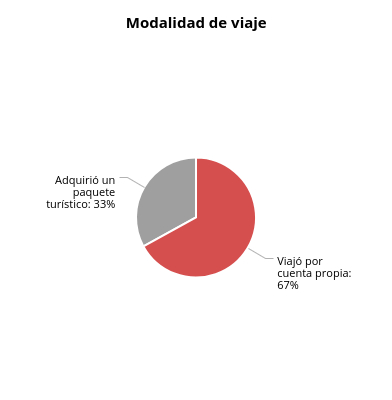
\includegraphics[scale=0.7]{Capitulo2/Figs/modalidad_viaje_extrajero.jpg}
    \caption{Porcentaje de modalidad de viaje de turista extranjero que visita Puno}
    Fuente: \citeA{2017PerfilExtranjero}
    \label{fig:modalidad_viaje_extrajero}
\end{figure}

\begin{figure}[!ht]
    \centering
    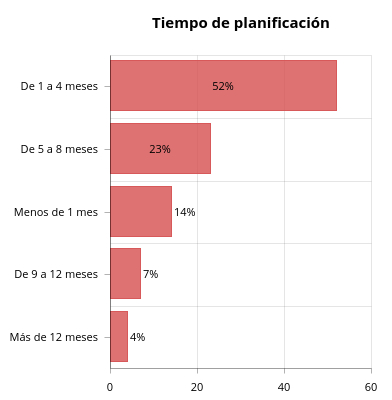
\includegraphics[scale=0.7]{Capitulo2/Figs/tiempo_planificacion_extranjero.jpg}
    \caption{Porcentaje de tiempo de planificación de viaje de turista extranjero que visita Puno}
    Fuente: \citeA{2017PerfilExtranjero}
    \label{fig:tiempo_planificacion_extranjero}
\end{figure}

De acuerdo a otro reporte publicado también publicado por PROMPERU titulado \cite{2017PerfilNacional} se observa que la información(ver Figura \ref{fig:tipo_infomacion_nacional}) que se busca más son las condiciones de las vias de acceso en un 56\%, 49 \%lugares turísticos para visitar, 41\% Costo del trasporte al lugar visitado, 38\% costos de alojamiento y sus características, por lo tanto se ve que una solución como la que proponemos ayudará en la toma de decisiones en la planificación de itinerarios en la región Puno.

\begin{figure}[!ht]
    \centering
    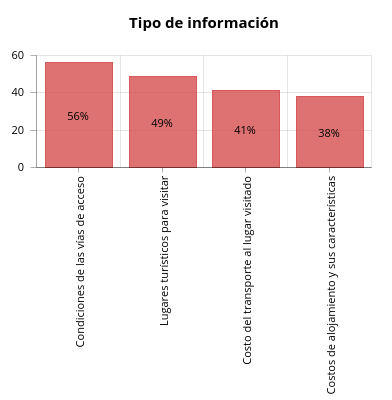
\includegraphics[scale=0.7]{Capitulo2/Figs/tipo_informacion_nacional.jpg}
    \caption{Porcentaje de tipo de información de vacionista nacional que visita Puno}
    Fuente: \citeA{2017PerfilNacional}
    \label{fig:tipo_infomacion_nacional}
\end{figure}

También al observar que los servicios de agencias de viajes ofrecen son transporte, alojamiento, alimentación, asistencia, etc. Y que los turistas prefieren opciones más personalizadas, en el trabajo que se realizará se considera que se hará un acercamiento a los servicios que brinda las agencias ya que como se puede observar en la Figura \ref{fig:tipo_infomacion_nacional} las información que buscan lo turistas son relacionados, combinado con la personalización.

La personalización es la palabra clave en el 2018 menciona \citeA{Estadisticas2018-2019} , donde también indica que:
“En 2018, la personalización es el lema al respecto de la experiencia del turista. (Skift, 2018)
Un 57\% de los turistas sienten que las marcas deberían adaptar su información acorde a las preferencias personales o conductas anteriores (Google/Phocuswright, 2017)
Si una marca de turismo adapta su información y experiencia general de la actividad en las preferencias personales o conductas anteriores, un 36\% de los turistas estaría dispuesto a pagar más por sus servicios.(Google/Phocuswright, 2017)”